\documentclass[german,10pt,a4paper]{article}

\usepackage{url}
\usepackage[hidelinks]{hyperref}
% \usepackage{fancyhdr}
\usepackage{fontspec}
\usepackage{csquotes}
\usepackage[ngerman]{babel}
\usepackage[colorinlistoftodos]{todonotes}
\usepackage[backend=biber,style=numeric]{biblatex}
\usepackage{graphicx}
\usepackage{float}
\usepackage{wrapfig}
\usepackage{amsmath}
\usepackage{amsfonts}
\usepackage{commath}
\usepackage{gensymb}
\usepackage{listings,xcolor,gnuplottex}
\usepackage[font={it}]{caption}
\usepackage{subcaption}
\usepackage{siunitx}
\usepackage{booktabs}
%\usepackage[german]{translator}
\pagestyle{headings}
\setcounter{secnumdepth}{3}
\setcounter{tocdepth}{3}

\selectlanguage{german}%
% Space savings:
\usepackage[top=5cm, left=2.5cm, right=2.5cm, bottom=3cm]{geometry}
\setlength\parindent{0pt}
% \usepackage[subtle]{savetrees}
\flushbottom
\raggedbottom
% Mathematica listening
\lstset{language=Mathematica} % mathmatica snippets
\lstset{basicstyle={\sffamily\footnotesize},
  numbers=left,
  numberstyle=\tiny\color{gray},
  numbersep=5pt,
  breaklines=true,
  captionpos={t},
  frame={lines},
  rulecolor=\color{black},
  framerule=0.5pt,
  columns=flexible,
  tabsize=2
}
%fancyer pararaphs:
\usepackage{titlesec}
\titleformat{\paragraph}{\normalfont\normalsize\bfseries}{}{}{}
\titlespacing{\paragraph}{0pt}{1em}{0pt}

%hack
\setcounter{tocdepth}{10}

\addbibresource{bib.bib}

\title{Akustische Richtungsbestimmung}
\author{Robin Heinemann\\ Jaro Habiger}
\date{\today}

\begin{document}
\begin{centering}
    Jugend forscht Arbeit
  	{\let\newpage\relax\maketitle}
  	\begin{figure}
  		\centering
  		{\large Erstellt im Schülerforschungszentrum Nordhessen}\\
  		\vspace{20pt}
  		\includegraphics[width=0.2\textwidth]{img/sfn}
  	\end{figure}
\end{centering}
\thispagestyle{empty}
\newgeometry{top=2.5cm, left=2.5cm, right=2.5cm, bottom=2cm}
\newpage
\tableofcontents

\iffalse

\fi

\thispagestyle{empty}

\newpage
\setcounter{page}{1}
% begin the content

\begingroup
\let\clearpage\relax
\section{Akustische Richtungsbestimmung} Der Mensch hat die Fähigkeit, direktional zu hören, also die Richtung zu bestimmen, aus der ein Geräusch kommt. Dies bringt ihm enorme Vorteile bei der Erkennung von gesprochener Sprache und bei anderen akustischen Aufgaben. Diese Fähigkeit auf eine technische Apparatur zu übertragen und die Vorteile des räumlichen Hörens auch für diese nutzbar zu machen, hätte viele Anwendungsgebiete, die unser alltägliches Leben erleichtern könnten.\\
Ein gutes Beispiel für eine solche Anwendung wäre ein Rettungsroboter, der hilfesuchende Menschen anhand von Hilferufen lokalisiert. Auch könnte man verschiedene Hilfsmittel für den Menschen konstruieren, die helfen Personen in verrauchten Umgebungen zu finden.
Weiterhin sind auch Anwendungen aus komplett anderen Anwendungsbereichen denkbar: So wäre es möglich eine Anwendung zu entwickeln, die die Richtungsinformationen verwendet, um Audiosignale zu filtern. Dadurch könnte man Anwendungen die störungsfreie Audiosignale benötigen, wie zum Bespiel Spracherkennung\cite{Spracherkennung}, verbessern.

\section{Bestehende Lösungen}
  Es gibt einige bestehende Ansätze, die die verschiedenen Aspekte des direktionalen Hörens auf eine technische Apparatur übertragen. Diesen begegnen wir in unserem alltäglichen Leben relativ häufig. Die einfachste Form eines solchen Verfahrens ist das Richtmikrofon. Dieses führt allerdings keine aktive Ortung durch, sondern kann lediglich in eine bestimmte Richtung besonders gut Schall aufnehmen. Um diese Fähigkeit für eine Richtungsbestimmung zu nutzen, müsste man also das Richtmikrofon drehen, oder es auf eine andere Weise aktiv nach der Schallquelle ausrichten. Ein weiterer Ansatz, dem wir in unserem alltäglichen Leben noch sehr viel häufiger begegnen, steckt in fast allen Mobiltelefonen. Diese filtern beim Telefonieren verschiedene Umgebungsgeräusche aus dem Mikrofonsignal, um die Sprachqualität zu verbessern. Die hierzu verwendeten Verfahren sind allerdings meist eher einfach gehalten und erlauben keine Bestimmung der Herkunftsrichtung eines Geräusches. Das Resultat dieses Verfahrens ähnelt sehr dem eines Richtmikrofons. Bei dieser Technik passiert ein Teil der Geräuschunterdrückung in der Signalverarbeitung, also nach der eigentlichen Schallwandlung durch das Mikrofon. Hierdurch unterscheidet sich dieser Ansatz deutlich von dem des Richtmikrofones. Allerdings können auch mithilfe dieser Störgeräuschunterdrückung noch keine Positionen ermittelt werden. Auch moderne Hörgeräte verwenden ein ähnliches Verfahren, welches allerdings auch bei einer weiteren Distanz zwischen Mikrofon und Schallquelle funktioniert, und der gesuchten Lösung somit näher kommt. Sowohl die Geräuschunterdrückung in Handys, als auch die Filtertechniken in Hörgeräten verwenden meist zwei oder drei Mikrofone.\\
     \begin{wrapfigure}{r}{0.5\textwidth}
     	\centering
        \includegraphics[width=0.5\linewidth]{img/akusticCamera}
     	\caption{Ein Beispiel für eine akustische Kamera \cite{camera}}
     	\label{fig:camera}
     \end{wrapfigure}
  Eine andere existierende Lösung ist die akustische Kamera (siehe Abb. \ref{fig:camera}). Sie wird dazu verwendet, lärmemittierende Positionen an Produkten zu finden, um diese optimieren zu können \cite{camera}. Die akustische Kamera verwendet allerdings bedeutend mehr Mikrofone als die anderen Verfahren. Einige Modelle verwenden mehr als 350 Mikrofone \cite{nmics}. Außerdem können bestehende akustische Kameras nicht in andere technische Kontexte eingebettet werden und sind so nicht universell einsetzbar. Da uns alle vorhandenen Lösungen nicht zufrieden gestellt haben, wollten wir ein eigenes Verfahren für die akustischen Richtungsbestimmung entwickeln, das schon mit einer geringen Anzahl von Mikrofonen eine komplette Richtungsbestimmung ermöglicht und leicht erweiterbar auf weitere Auswertungsschritte ist.

\section{Konzept}
Bei der Entwicklung unseres neuen Verfahren zur Richtungsbestimmung haben wir uns stark am menschlichen Gehör und seiner Fähigkeit des Richtungshörens orientiert. Da beim menschlichen Gehör verschiedene Verarbeitungssstufen durchlaufen werden, ist auch unsere Software modular aufgebaut (siehe Tabelle \ref{analog}). Nachfolgend werden die einzelnen Module in der Reihenfolge, in der das Signal sie durchläuft, beschrieben. 
Um unser Konzept umzusetzen und zu evaluieren, haben wir uns entschlossen, einerseits eine Computersimulation zu schreiben und andererseits mithilfe einer realen Messapparatur zu überprüfen, ob unser Verfahren auch in der Echtwelt verwendbar ist. Der reale Aufbau soll zuerst in einer Schallkammer, also einem Raum mit wenigen akustischen Störquellen von außen und mit wenigen akustischen Reflexionen an den Wänden, und erst danach unter Einfluss von Störungen getestet werden. Dieses Vorgehen hat den Vorteil, dass man zuerst die Theorie entwickeln kann, und danach die Theorie und ihre Implementation in den verschiedenen Schritten zum Endprodukt immer weiter an Realwelteffekte, wie z.B. Rauschen, anpassen kann. Auch hierbei hilft der modulare Aufbau, da so möglichst viele Programmteile sowohl in der Simulation, als auch in realen Aufbauten verwendet werden können.
\begin{table}[h]
	\centering
    \begin{tabular}{ll}
		Mensch            & Maschine                                   \\ \hline
        Ohren             & Mikrofonarray                              \\
        Gehirn            & Computeralgorithmus                        \\
		Haarzellen im Ohr & Fourier Transformation                     \\
		Selektives Hören  & Weiterverarbeitung durch Programme Dritter
	\end{tabular}
	\caption{Die Analogie zwischen dem menschlichen Gehör und unserem Verfahren}
	\label{analog}
\end{table}
Unser Konzept sieht vier Module vor, welche über TCP/IP und Websockets verbunden sind. Dies sind Standards, mit denen über ein Computernetzwerk Daten ausgetauscht werden können \cite{tcp} \cite{websockets}. Diese beiden Protokolle sind sehr zuverlässig und lange erprobt. Außerdem garantieren diese, dass alle Daten in der Reihenfolge, in der sie losgeschickt werden, ankommen. Die Verwendung von Netzwerkprotokollen hat den Vorteil, dass die Module nicht unbedingt auf demselben Computer ausgeführt werden müssen und so der Rechenaufwand bei Bedarf auf mehrere Computer verteilt werden kann.

\subsection{Modul 1: Eingabe/Aufnahme}
Das erste Modul in dieser Kette stellt die Rohdaten für die weitere Verarbeitung bereit. Diese  können entweder von einer Gruppe real existierender Mikrofone stammen oder, im Falle der Simulation, die Signale einer Gruppe simulierter Mikrofone, die simulierte Schallquellen aufnehmen, sein. Dieses Modul entspricht dem menschlichen Ohr und seiner Aufgabe, den Schall aufzunehmen. 

\subsection{Modul 2: Signal nach Frequenzen aufteilen}
Im zweiten Modul der Kette wird das Signal, welches aus dem ersten Modul stammt, in die einzelnen im Signal enthaltenen Wellen aufgeteilt, also von einer zeitaufgelösten Form in ein frequenzaufgelöstes Signal umgewandelt. Nach diesem Schritt liegt also für jede Frequenz eine Amplitude und eine Phase vor. Dieser Schritt wird im menschlichen Ohr durch eine mechanische Konstruktion, die verschiedene Haarzellen für verschiedene Frequenzen anregt, vorgenommen. Unser technisches Verfahren verwendet hierzu die Fouriertransformation. Diese Transformation hat den Vorteil, dass jede Frequenz mit ihrer zugehörigen Amplitude und Phase einzeln analysiert werden kann. 
In diesem Modul werden außerdem Frequenzen, welche nicht oder nur sehr leise in dem Eingangssignal vorkommen, herausgefiltert, um das Rauschen und den benötigten Rechenaufwand in den nächsten Modulen zu verringern.

\subsection{Modul 3: Richtungsbestimmung}
Das nächste Modul empfängt die Daten des vorherigen Moduls und errechnet zunächst für jede Frequenz aus den transformierten Daten den Gangunterschied zwischen den Signalen der Mikrofone. Aus diesen werden dann die möglichen Ursprungsrichtungen der einzelnen Sinusschwingung ermittelt. Da dieser Vorgang für jede Frequenz einzeln vorgenommen wird können auch mehrere Schallquellen mit unterschiedlichen Frequenzen gleichzeitig untersucht werden. Im menschlichen Gehör wird diese Richtungsbestimmung im Gehirn vorgenommen.

\subsection{Modul 4: Ausgabe}
Das letzte Modul in der Signalkette ist die Ausgabe. Sie bekommt die fertig gruppierten Messergebnisse über eine Websocket-Verbindung und bereitet sie für den Nutzer auf. Dieses Modul kann auf die jeweilige Anwendung angepasst werden und es können mehrere Output-Module mit dem gleichen Richtungsmodul verbunden werden. Hier kann dann die Endanwendung, die das Richtungshören verwenden möchte ``angeschlossen'' werden. Der Mensch kann sich zum Beispiel mithilfe der bestimmten Richtungen auf einzelne Schallquellen konzentrieren und andere Geräusche ausblenden.
\section{Umsetzung der einzelnen Module} \todo{Jaro: Bleibt, Ortung -> Richtung}
      \subsection{Simulation (Modul 1)}
      \subsection{Hardware (Modul 1)}
      \subsubsection{Mikrofone}
      \subsubsection{Audio Interface}
      \subsubsection{Software}
      \subsection{Fourier-Transformation (Modul 2)}
      \subsection{Ortungsmodul (Modul 3)}
      \subsection{Ausgabemodul (Modul 4)}
      \subsection{Testen der einzelnen Module}

  \section{Eindimensionale Richtungsbestimmung} \todo{Robin: Bleibt, Ortung -> Richtung}
  Um den Algorithmus, der aus den Phasendifferenzen den Ort zurückrechnet zu entwickeln haben wir mit der
einfachsten Stufe der Ortung, die eindimensionale Ortung, angefangen:
    \begin{figure}
        \centering
        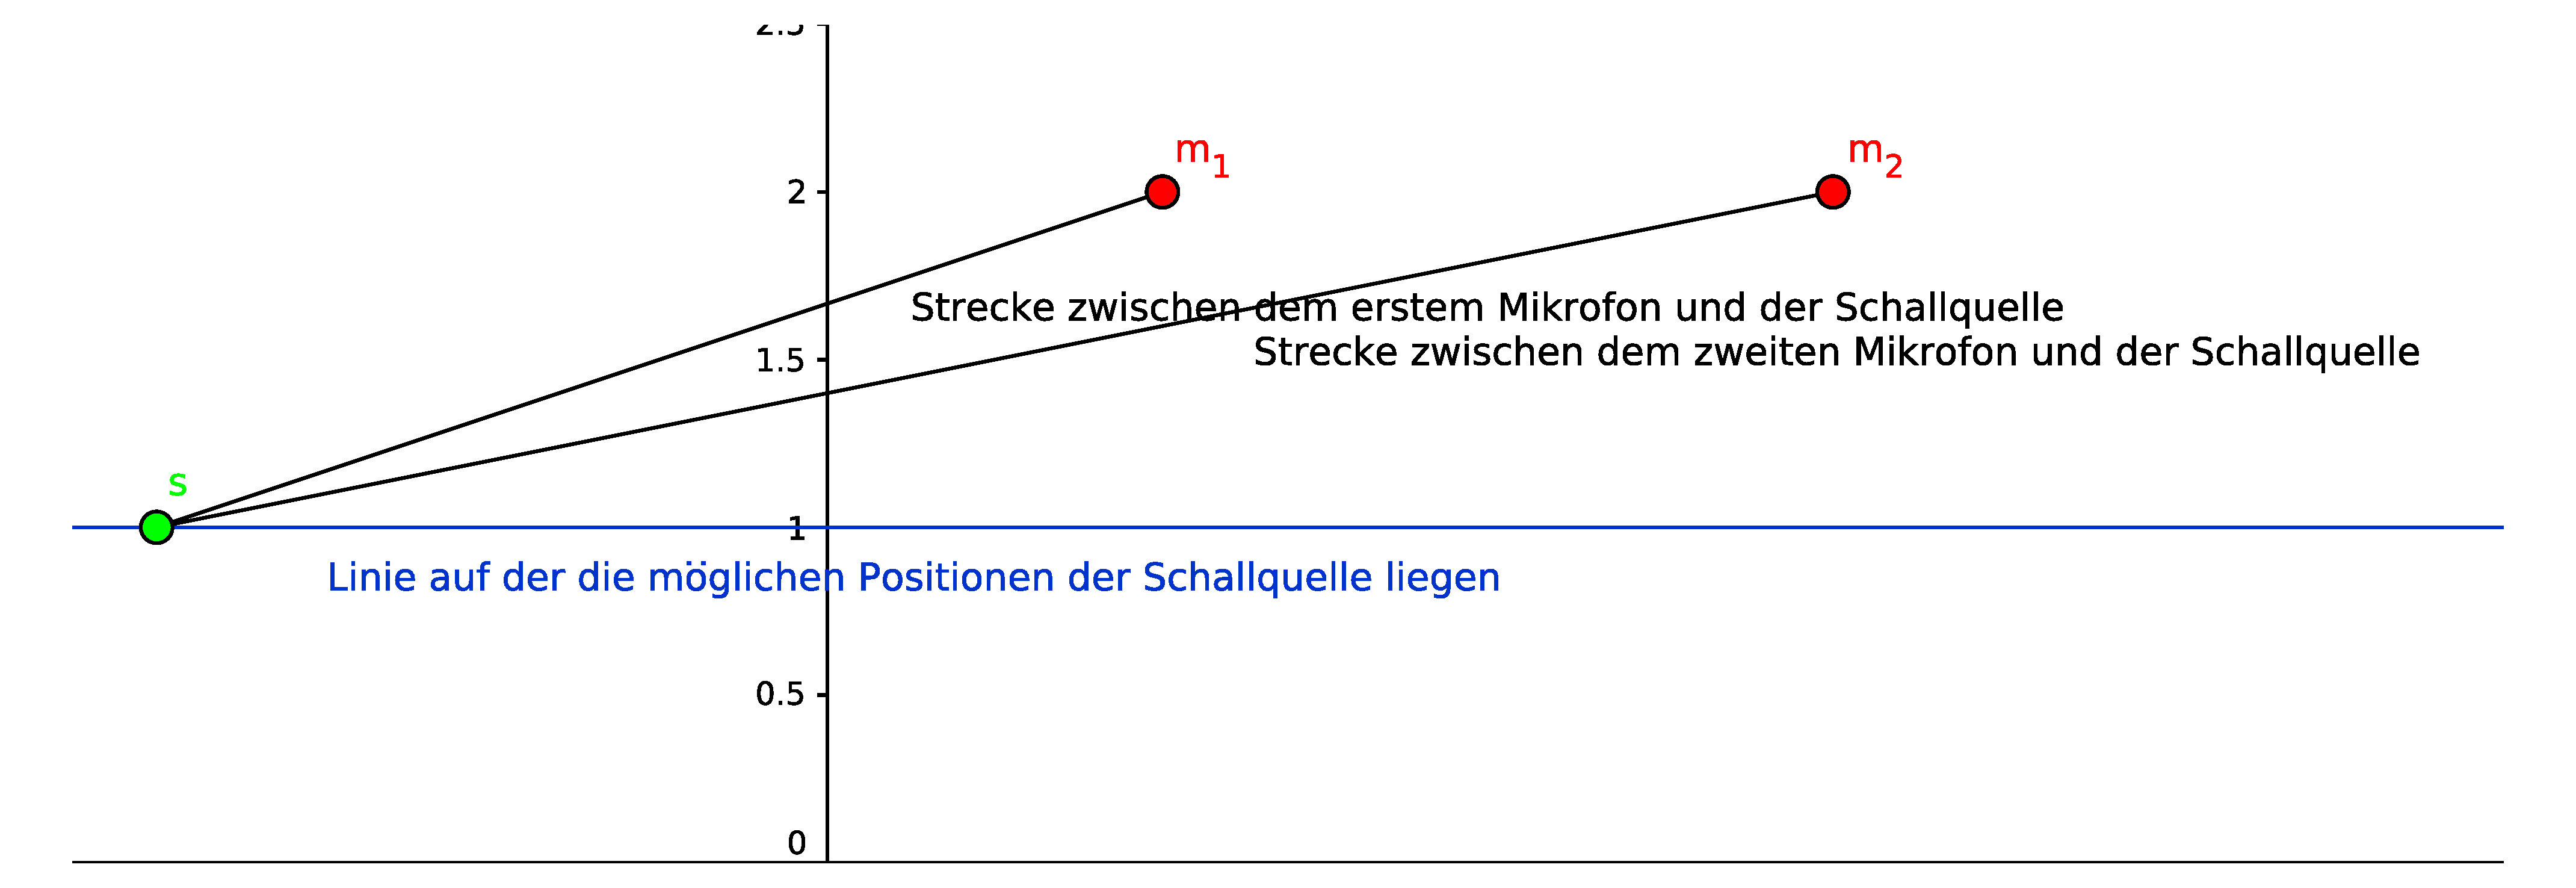
\includegraphics[width=\linewidth]{skizze1d}
        \caption{Skizze einer eindimensionalen Ortung}
    \end{figure}

  \section{Zweidimensionale Ortung} \todo{Robin: Bleibt, Ortung -> Richtung, analytisch -> numerisch}
      \subsection{Erweiterung der Theorie}
      \subsection{Analytisches Lösen des gleichungssystems}

\section{Dreidimensionale Richtungsbestimmung}
\subsection{Erweiterung der Theorie}
Um die Richtungsbestimmung dann auf drei Dimensionen zu erweitern, müssen zuerst die Ortsvektoren der Mikrofone und der der Schallquelle auf drei Dimensionen erweitert werden: $$\vec{m}_i = \begin{pmatrix}
m_{ix} \\
m_{iy} \\
m_{iz}
\end{pmatrix} \quad\quad
\vec{s} = \begin{pmatrix}
{s_x} \\
{s_y} \\
{s_z}
\end{pmatrix}$$
Mit den angepassten Ortsvektoren erhält man eine neue Formel für die Abstandsberechnung zwischen einem Mikrofon und der Schallquelle:
$$\abs{\vec{m}_i - \vec{s}} = \sqrt{{(m_{ix} - s_x)}^2 + {(m_{iy} - s_y)}^2 + {(m_{i_z} - s_z)}^2}$$
Man erhält eine weitere Unbekannte, $m_{iz}$. Dadurch wird für die dreidimensionale Ortung ein viertes Mikrofon benötigt. Mit dem vierten Mikrofon erhält man eine dritte Gleichung, die den Gangunterschied zwischen dem ersten und dem vierten Mikrofon enthält, dadurch wird das Gleichungssystem wieder eindeutig lösbar:
$$\left|\begin{array}{c}
\abs{\vec{m}_1 - \vec{s}} - \abs{\vec{m}_2 - \vec{s}} = \Delta{x_{12}} \\
\abs{\vec{m}_1 - \vec{s}} - \abs{\vec{m}_3 - \vec{s}} = \Delta{x_{13}} \\
\abs{\vec{m}_1 - \vec{s}} - \abs{\vec{m}_4 - \vec{s}} = \Delta{x_{14}}
\end{array}\right|$$
$$\left|\begin{array}{c}
\sqrt{{(m_{1x} - s_x)}^2 + {(m_{1y} - s_y)}^2} - \sqrt{{(m_{2x} - s_x)}^2 + {(m_{2y} - s_y)}^2 + {(m_{2_z} - s_z)}^2} = \Delta{x_{12}} \\
\sqrt{{(m_{1x} - s_x)}^2 + {(m_{1y} - s_y)}^2} - \sqrt{{(m_{3x} - s_x)}^2 + {(m_{3y} - s_y)}^2 + {(m_{3_z} - s_z)}^2} = \Delta{x_{13}} \\
\sqrt{{(m_{1x} - s_x)}^2 + {(m_{1y} - s_y)}^2} - \sqrt{{(m_{4x} - s_x)}^2 + {(m_{4_y} - s_y)}^2 + {(m_{4_z} - s_z)}^2} = \Delta{x_{14}}
\end{array}\right|$$
\subsection{Numerische Lösung des Gleichungssystems mit Singulärwertzerlegung und Gauss-Markow Algorithmus}
Schon für zwei Dimensionen ist die analytische Lösung des Gleichungssystem sehr kompliziert. Für drei Dimensionen ist die Formel der Lösung in Textform über 300Mb groß. Dadurch können wir sie nur durch Einschränkung der Mikrofon-Positionen verwenden. Um diese Einschränkung zu umgehen, lösen wir das Gleichungssystem numerisch. Dazu verwenden wir das mehrdimensionale Newtonverfahren. Hierbei gehen wir von einer Startposition $\vec{s}_0$ aus, die iterativ verbessert wird. Als Startposition haben wir das Zentrum der Mikrofone gewählt. Für den Iteratiosvektoren erhält man eine neue Formel für die Abstandsberechnung zwischen einem Mikrofon und der Schallquelle:
$$\abs{\vec{m}_i - \vec{s}} = \sqrt{{(m_{ix} - s_x)}^2 + {(m_{iy} - s_y)}^2 + {(m_{i_z} - s_z)}^2}$$
Man erhält eine weitere nsschritt $i$ erhält man die neue Positionen mit $\vec{s}_{i + 1} = \vec{s}_i + \vec{\Delta{s}}_i$. Das Gleichungssystem für die dreidimensionale Ortung lässt sich umschreiben zu:
$$\left|\begin{array}{c}
\sqrt{(m_{1x} - s_x)^2 + (m_{1y} - s_y)^2 + (m_{1_z} - s_z)^2} - d = 0 \\
\sqrt{(m_{2x} - s_x)^2 + (m_{2y} - s_y)^2 + (m_{2_z} - s_z)^2} - d = \Delta{x_{12}} \\
\sqrt{(m_{3x} - s_x)^2 + (m_{3y} - s_y)^2 + (m_{3_z} - s_z)^2} - d = \Delta{x_{13}} \\
\sqrt{(m_{4x} - s_x)^2 + (m_{4y} - s_y)^2 + (m_{4_z} - s_z)^2} - d = \Delta{x_{14}} \\
\end{array}\right|$$
Um dieses Gleichungssystem mit dem Newtonverfahren zu lösen wird es mit der Taylorentwicklung bis zur ersten Ordung linearisiert:
$$\left|\begin{array}{c}
-r_{1_{ca}} = \frac{s_{ix} - m_{1x}}{r_{1_{ca}}} \cdot \vec{\Delta{s}}_{ix} + \frac{s_{iy} - m_{1y}}{r_{1_{ca}}} \cdot \vec{\Delta{s}}_{iy} + \frac{s_{i_z} - m_{1_z}}{r_{1_{ca}}} \cdot \vec{\Delta{s}}_{i_z} - d \\
\Delta{x_{12}} - r_{2_{ca}} = \frac{s_{ix} - m_{2x}}{r_{2_{ca}}} \cdot \vec{\Delta{s}}_{ix} + \frac{s_{iy} - m_{2y}}{r_{2_{ca}}} \cdot \vec{\Delta{s}}_{iy} + \frac{s_{i_z} - m_{2_z}}{r_{2_{ca}}} \cdot \vec{\Delta{s}}_{i_z} - d \\
\Delta{x_{13}} - r_{3_{ca}} = \frac{s_{ix} - m_{3x}}{r_{3_{ca}}} \cdot \vec{\Delta{s}}_{ix} + \frac{s_{iy} - m_{3y}}{r_{3_{ca}}} \cdot \vec{\Delta{s}}_{iy} + \frac{s_{i_z} - m_{3_z}}{r_{3_{ca}}} \cdot \vec{\Delta{s}}_{i_z} - d \\
\Delta{x_{14}} - r_{4_{ca}} = \frac{s_{ix} - m_{4x}}{r_{4_{ca}}} \cdot \vec{\Delta{s}}_{ix} + \frac{s_{iy} - m_{4y}}{r_{4_{ca}}} \cdot \vec{\Delta{s}}_{iy} + \frac{s_{i_z} - m_{4_z}}{r_{4_{ca}}} \cdot \vec{\Delta{s}}_{i_z} - d \\
\end{array}\right|$$
$$r_{i_{ca}} = \sqrt{(m_{ix} - s_{ix})^2 + (m_{iy} - s_{iy})^2 + (m_{i_z} - s_{i_z})^2}$$

$$
\begin{pmatrix}
\vec{\Delta{s}}_{ix} \\
\vec{\Delta{s}}_{iy} \\
\vec{\Delta{s}}_{iz} \\
                d \\
\end{pmatrix}
=
{\begin{pmatrix}
\frac{s_{ix} - m_{1x}}{r_{1_{ca}}} & \frac{s_{iy} - m_{1y}}{r_{1_{ca}}} & \frac{s_{i_z} - m_{1_z}}{r_{1_{ca}}} & -1 \\
\frac{s_{ix} - m_{2x}}{r_{2_{ca}}} & \frac{s_{iy} - m_{2y}}{r_{2_{ca}}} & \frac{s_{i_z} - m_{1_z}}{r_{2_{ca}}} & -1 \\
\frac{s_{ix} - m_{3x}}{r_{3_{ca}}} & \frac{s_{iy} - m_{3y}}{r_{3_{ca}}} & \frac{s_{i_z} - m_{1_z}}{r_{3_{ca}}} & -1 \\
\frac{s_{ix} - m_{4x}}{r_{4_{ca}}} & \frac{s_{iy} - m_{4y}}{r_{4_{ca}}} & \frac{s_{i_z} - m_{1_z}}{r_{4_{ca}}} & -1 \\
\end{pmatrix}}^{-1}
\cdot
\begin{pmatrix}
-r_{1_{ca}}\\

\Delta{x_{12}} - r_{2_{ca}}\\
\Delta{x_{13}} - r_{3_{ca}}\\
\Delta{x_{14}} - r_{4_{ca}}
\end{pmatrix}
$$
Für die Berechnung der Inverse der Matrix gibt es viele verschiedene Methoden, wir benutzen die Singulärwertszerlegung. Die numerische Lösung des Gleichungssystems benötigt eine initiale Position, für die die Mitte der Mikrofone verwendet wird. Wenn allerdings bereits eine alte Position für die vorliegende Frequenz bekannt ist, wird diese alte Position als Startwert der Iteration verwendet, da dadurch, wenn sich die Position der Schallquelle nicht zu sehr geändert hat, die Iteration schneller konvergiert. Als Konvergenzkriterium verwenden wir $\abs{\vec{\Delta{s}}_i} < 0.0001\mathrm{m}$. Da das Newtonverfahren keine garantierte Konvergenz hat, wird die Iteration nach $50$ Iterationsschitten abgebrochen.
Ein Vorteil der numerischen Lösung ist, dass sie leicht auf beliebig viele Mikrofone erweitert werden kann. Das Gleichungssystem wird überbestimmt, wenn man mehr als vier Mikrofone verwendet, aber indem man die Methode der kleinsten Quadrate auf die Berechnung von $\vec{\Delta{s}}_i$ anwendet, erhält man den Ort, an dem die Summe der Fehlerquadrate für alle Mikrofone am geringsten ist, es also am wahrscheinlichsten ist, dass sich die Schallquelle wirklich dort befindet. Die Least Squares Lösung entspricht für unser Problem, nach dem Gauss-Markow-Theorem einem minimalvarianten linearen erwatungstreuen Schätzer. Außerdem kann man mit mehr Mikrofonen die Richtungsbestimmung auch unabhängig von der Schallgeschwindigkeit machen, denn diese kann als eine weitere Variable eingeführt werden.
\subsection{Zusammenfassen von ähnlichen Richtungen}
Signale in der Echtwelt bestehen aus vielen verschiedenen Frequenzen, dadurch erhält man anstatt einer Richtung für eine Schallquelle, wie eine sprechender Mensch, nicht nur eine Richtung, sondern viele ähnliche Richtungen. Um die ermittelten Richtungen eindeutiger zu machen fassen wir deswegen diese ähnliche Richtungen zusammen. Dazu verwenden wir ein agglomeratives Clusterverfahren mit der Summe der minimalen Winkel zwischen zwei Richtungen als Unähnlichkeit. Von jeder Frequenz werden die letzten zehn Richtungen gespeichert und diese fließen mit in die Clusterbildung mit ein. Um geringe Änderungen in der Richtung auszugleichen wird außerdem ein laufendes Mittel der Richtung für jede Frequenz über drei Richtungen gebildet. Die Richtung eines Clusters wird über ein nach dem Amplituden gewichtetes Mittel aus allen zu dem Cluster gehörenden Richtungen berechnet.
\section{Evaluation}
Um unser Verfahren zur Richtungsbestimmung zu testen und die Genauigkeit zu bestimmen, haben wir es in Simulation und Echtwelt evaluiert. Dabei haben wir die Abweichung der Richtungsbestimmung für verschiedene Richtungen und Frequenzen bestimmt.
\subsection{Audiosimulation}
Zunächst haben wir unser Verfahren in der Simulation getestet, da diese automatisierte Tests ermöglicht und somit leicht sehr viele verschiedene Richtungen/Frequenzen getestet werden können. Dabei haben wir die Schallquellen für verschiedene Radien auf einer Kugeloberfläche positioniert. Der Tetraeder wurde mit $0.28m$ Kantenlänge simuliert, dies entspricht dem Tetraeder, den wir auch in der Echtwelt gebaut haben. Die Schallquellen wurden mit einer $500Hz$ Sinusschwingung simuliert.
\begin{figure}[H]
  \centering
  % GNUPLOT: LaTeX picture with Postscript
\begingroup
  \makeatletter
  \providecommand\color[2][]{%
    \GenericError{(gnuplot) \space\space\space\@spaces}{%
      Package color not loaded in conjunction with
      terminal option `colourtext'%
    }{See the gnuplot documentation for explanation.%
    }{Either use 'blacktext' in gnuplot or load the package
      color.sty in LaTeX.}%
    \renewcommand\color[2][]{}%
  }%
  \providecommand\includegraphics[2][]{%
    \GenericError{(gnuplot) \space\space\space\@spaces}{%
      Package graphicx or graphics not loaded%
    }{See the gnuplot documentation for explanation.%
    }{The gnuplot epslatex terminal needs graphicx.sty or graphics.sty.}%
    \renewcommand\includegraphics[2][]{}%
  }%
  \providecommand\rotatebox[2]{#2}%
  \@ifundefined{ifGPcolor}{%
    \newif\ifGPcolor
    \GPcolorfalse
  }{}%
  \@ifundefined{ifGPblacktext}{%
    \newif\ifGPblacktext
    \GPblacktexttrue
  }{}%
  % define a \g@addto@macro without @ in the name:
  \let\gplgaddtomacro\g@addto@macro
  % define empty templates for all commands taking text:
  \gdef\gplbacktext{}%
  \gdef\gplfronttext{}%
  \makeatother
  \ifGPblacktext
    % no textcolor at all
    \def\colorrgb#1{}%
    \def\colorgray#1{}%
  \else
    % gray or color?
    \ifGPcolor
      \def\colorrgb#1{\color[rgb]{#1}}%
      \def\colorgray#1{\color[gray]{#1}}%
      \expandafter\def\csname LTw\endcsname{\color{white}}%
      \expandafter\def\csname LTb\endcsname{\color{black}}%
      \expandafter\def\csname LTa\endcsname{\color{black}}%
      \expandafter\def\csname LT0\endcsname{\color[rgb]{1,0,0}}%
      \expandafter\def\csname LT1\endcsname{\color[rgb]{0,1,0}}%
      \expandafter\def\csname LT2\endcsname{\color[rgb]{0,0,1}}%
      \expandafter\def\csname LT3\endcsname{\color[rgb]{1,0,1}}%
      \expandafter\def\csname LT4\endcsname{\color[rgb]{0,1,1}}%
      \expandafter\def\csname LT5\endcsname{\color[rgb]{1,1,0}}%
      \expandafter\def\csname LT6\endcsname{\color[rgb]{0,0,0}}%
      \expandafter\def\csname LT7\endcsname{\color[rgb]{1,0.3,0}}%
      \expandafter\def\csname LT8\endcsname{\color[rgb]{0.5,0.5,0.5}}%
    \else
      % gray
      \def\colorrgb#1{\color{black}}%
      \def\colorgray#1{\color[gray]{#1}}%
      \expandafter\def\csname LTw\endcsname{\color{white}}%
      \expandafter\def\csname LTb\endcsname{\color{black}}%
      \expandafter\def\csname LTa\endcsname{\color{black}}%
      \expandafter\def\csname LT0\endcsname{\color{black}}%
      \expandafter\def\csname LT1\endcsname{\color{black}}%
      \expandafter\def\csname LT2\endcsname{\color{black}}%
      \expandafter\def\csname LT3\endcsname{\color{black}}%
      \expandafter\def\csname LT4\endcsname{\color{black}}%
      \expandafter\def\csname LT5\endcsname{\color{black}}%
      \expandafter\def\csname LT6\endcsname{\color{black}}%
      \expandafter\def\csname LT7\endcsname{\color{black}}%
      \expandafter\def\csname LT8\endcsname{\color{black}}%
    \fi
  \fi
    \setlength{\unitlength}{0.0500bp}%
    \ifx\gptboxheight\undefined%
      \newlength{\gptboxheight}%
      \newlength{\gptboxwidth}%
      \newsavebox{\gptboxtext}%
    \fi%
    \setlength{\fboxrule}{0.5pt}%
    \setlength{\fboxsep}{1pt}%
\begin{picture}(9360.00,7200.00)%
    \gplgaddtomacro\gplbacktext{%
      \colorrgb{0.50,0.50,0.50}%
      \put(1240,1722){\makebox(0,0){\strut{}$-2$}}%
      \colorrgb{0.50,0.50,0.50}%
      \put(1634,1609){\makebox(0,0){\strut{}$-1.5$}}%
      \colorrgb{0.50,0.50,0.50}%
      \put(2027,1496){\makebox(0,0){\strut{}$-1$}}%
      \colorrgb{0.50,0.50,0.50}%
      \put(2421,1383){\makebox(0,0){\strut{}$-0.5$}}%
      \colorrgb{0.50,0.50,0.50}%
      \put(2815,1270){\makebox(0,0){\strut{}$0$}}%
      \colorrgb{0.50,0.50,0.50}%
      \put(3208,1158){\makebox(0,0){\strut{}$0.5$}}%
      \colorrgb{0.50,0.50,0.50}%
      \put(3602,1045){\makebox(0,0){\strut{}$1$}}%
      \colorrgb{0.50,0.50,0.50}%
      \put(3995,932){\makebox(0,0){\strut{}$1.5$}}%
      \colorrgb{0.50,0.50,0.50}%
      \put(4389,819){\makebox(0,0){\strut{}$2$}}%
      \csname LTb\endcsname%
      \put(2427,975){\makebox(0,0){\strut{}x [m]}}%
      \colorrgb{0.50,0.50,0.50}%
      \put(4569,860){\makebox(0,0){\strut{}$-2$}}%
      \colorrgb{0.50,0.50,0.50}%
      \put(4797,1055){\makebox(0,0){\strut{}$-1.5$}}%
      \colorrgb{0.50,0.50,0.50}%
      \put(5024,1251){\makebox(0,0){\strut{}$-1$}}%
      \colorrgb{0.50,0.50,0.50}%
      \put(5251,1446){\makebox(0,0){\strut{}$-0.5$}}%
      \colorrgb{0.50,0.50,0.50}%
      \put(5479,1641){\makebox(0,0){\strut{}$0$}}%
      \colorrgb{0.50,0.50,0.50}%
      \put(5706,1837){\makebox(0,0){\strut{}$0.5$}}%
      \colorrgb{0.50,0.50,0.50}%
      \put(5933,2032){\makebox(0,0){\strut{}$1$}}%
      \colorrgb{0.50,0.50,0.50}%
      \put(6161,2228){\makebox(0,0){\strut{}$1.5$}}%
      \colorrgb{0.50,0.50,0.50}%
      \put(6388,2423){\makebox(0,0){\strut{}$2$}}%
      \csname LTb\endcsname%
      \put(6152,1470){\makebox(0,0){\strut{}y [m]}}%
      \colorrgb{0.50,0.50,0.50}%
      \put(1180,1817){\makebox(0,0)[r]{\strut{}$-2$}}%
      \colorrgb{0.50,0.50,0.50}%
      \put(1180,2208){\makebox(0,0)[r]{\strut{}$-1.5$}}%
      \colorrgb{0.50,0.50,0.50}%
      \put(1180,2599){\makebox(0,0)[r]{\strut{}$-1$}}%
      \colorrgb{0.50,0.50,0.50}%
      \put(1180,2989){\makebox(0,0)[r]{\strut{}$-0.5$}}%
      \colorrgb{0.50,0.50,0.50}%
      \put(1180,3380){\makebox(0,0)[r]{\strut{}$0$}}%
      \colorrgb{0.50,0.50,0.50}%
      \put(1180,3770){\makebox(0,0)[r]{\strut{}$0.5$}}%
      \colorrgb{0.50,0.50,0.50}%
      \put(1180,4161){\makebox(0,0)[r]{\strut{}$1$}}%
      \colorrgb{0.50,0.50,0.50}%
      \put(1180,4552){\makebox(0,0)[r]{\strut{}$1.5$}}%
      \colorrgb{0.50,0.50,0.50}%
      \put(1180,4942){\makebox(0,0)[r]{\strut{}$2$}}%
      \csname LTb\endcsname%
      \put(382,3380){\makebox(0,0){\strut{}z [m]}}%
      \put(6522,4854){\makebox(0,0)[l]{\strut{}Ausschnitt (vergrößert)}}%
    }%
    \gplgaddtomacro\gplfronttext{%
      \csname LTb\endcsname%
      \put(5725,6696){\makebox(0,0)[r]{\strut{}getestete Positionen (für r=1.4m)}}%
      \csname LTb\endcsname%
      \put(5725,6696){\makebox(0,0)[r]{\strut{}getestete Positionen (für r=1.4m)}}%
    }%
    \gplgaddtomacro\gplbacktext{%
    }%
    \gplgaddtomacro\gplfronttext{%
    }%
    \gplbacktext
    \put(0,0){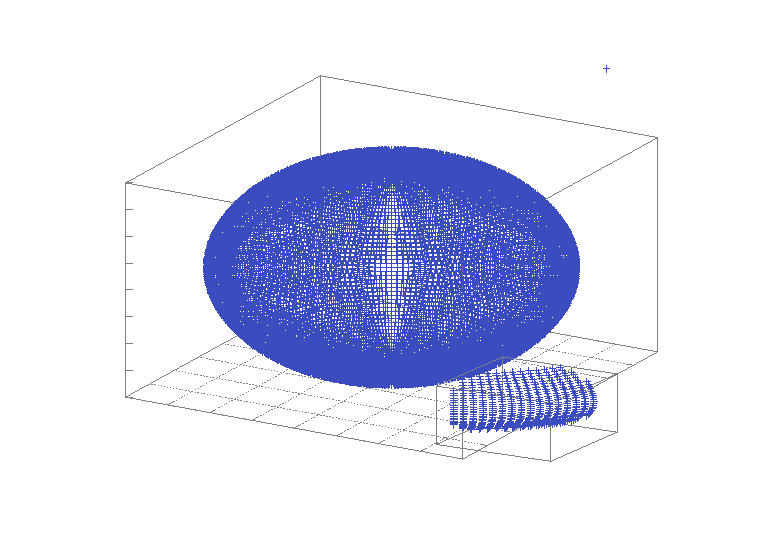
\includegraphics{img/tested_positions_zoom}}%
    \gplfronttext
  \end{picture}%
\endgroup

  \caption{Visualisierung der getesteten Positionen}
  \label{fig:pos}
\end{figure}
Für jeden getesteten Radius haben wir Punkte auf der Kugeloberfläche in 2° Auflösung, also insgesamt 32400 Positionen, getestet.
\begin{figure}[H]
  \centering
  \input{img/pos_sweep}
  \caption{Genauigkeit für verschiedene Abstände}
  \label{fig:pos_sweep}
\end{figure}
Bei einem Radius von $0.25m$ gibt es einen Ausreißer mit $4.0^\circ \pm 0.4^\circ$, da sich die Positionen innerhalb des Tetraeders befinden. Bis $1.75m$ bleibt die Abweichung deutlich unter $2^\circ$, ist also deutlich besser als beim Menschen. Dieser kann auf sehr kurze Distanzen zwischen $10cm$ und $40cm$ gerade einmal mit $3^\circ$ Genauigkeit die Richtung bestimmen. \cite{middlebrooks1991sound}
Um die Abhängigkeit der Genauigkeit der Richtungsbestimmung von der Frequenz zu untersuchen, haben wir die Schallquellen wieder auf einer Kugeloberfläche mit $2^\circ$ Auflösung platziert und haben anstelle des Radius die Frequenz variiert. Für den Radius haben wir $1.4m$ gewählt.
\begin{figure}[H]
  \centering
  \input{img/freq_sweep}
  \caption{Genauigkeit für verschiedene Frequenzen}
  \label{fig:freq_seep}
\end{figure}
Man sieht, dass die Genauigkeit der Richtungsbestimmung (fast) unabhängig von der Frequenz der Schallquelle ist. Für Frequenzen über $675Hz$ ist die Bedingung, dass die Abstände der Mikrofone kleiner als die halbe Wellenlänge sein muss, nicht mehr erfüllt.
\subsection{Echtwelt}
In unseren Simulationen hat sich gezeigt, dass unser Verfahren sehr genau arbeitet. Um zu untersuchen, wie genau es unter dem Einfluss von Störungen und mit den Fehlern durch die Aufnahme mit Mikrofonen arbeitet, haben wir für acht verschiedene Positionen der Schallquelle die Abweichung der Richtung bestimmt. Diese Messung haben wir in einem mit speziellem Schaumstoff~\cite{BASOTECT} ausgekleideten Raum durchgeführt, um Störungen wie Reflexionen, in der Testphase, zu minimieren. Der Lautsprecher war jeweils $0.75m$ von dem Zentrum der Mikrofone entfernt.
\begin{figure}[H]
  \centering
  \resizebox{!}{0.55\textwidth}{\input{img/real}}
  \caption{Genauigkeit in der Echtwelt}
  \label{fig:real}
\end{figure}
\begin{figure}[H]
  \centering
  \includegraphics[width=.5\textwidth]{img/pos_1}
  \caption{Versuchsaufbau zur Messung der Genauigkeit der Richtungsbestimmung in der Schallkammer}
  \label{fig:real_reral}
\end{figure}
Für die acht verschiedenen Richtungen hatte die Richtungsbestimmung eine Genauigkeit von $3.9^\circ \pm 0.13^\circ$. Allerdings hatte der Lautsprecher bei dem von uns gewählten Abstand eine Winkelgröße von $3.2^\circ$, genauer als diese kann die Richtungsbestimmung also nicht sein. Die Richtungsbestimmung mit unserem Verfahren ist also auch in der Echtwelt genauer als beim Menschen.

\subsection{Alltagstest}
Um die Verwendbarkeit unseres Verfahren auch außerhalb einer Schallkammer zu testen, haben wir die Richtungsbestimmung zweier sich unterhaltender Personen untersucht.\\
\begin{minipage}{0.49\linewidth}
  \begin{figure}[H]
    \centering
    \includegraphics[width=\textwidth]{img/real_real_data}
    \caption{Bestimmte Richtungen}
    \label{fig:real_real_data}
  \end{figure}
\end{minipage}\hfill
\todo{neue Abbildung}
\begin{minipage}{0.49\linewidth}
  \begin{figure}[H]
    \centering
    \includegraphics[width=\textwidth]{img/real_real}
    \caption{Tatsächliche Position}
    \label{fig:real_real}
  \end{figure}
\end{minipage}
\vspace{10pt}
\\
Man kann erkennen, dass die mit unserem Verfahren bestimmte Richtung sehr gut mit der tatsächlichen Richtung übereinstimmt und es auch nur eine sehr geringe Streuung der Richtung gibt. Dies zeigt, dass unser Verfahren auch für Echtwelt Situationen, bei denen Störungen wie Reflexionen auftreten, gut geeignet ist.


%\addcontentsline{toc}{subsection}{\protect\numberline{8.2} Realwelt}
%\addcontentsline{toc}{subsection}{\protect\numberline{8.3} Alltagstest}

\section{Ausblick} \todo{Beide: Neu, 8mics ja, 38 verschweigen}


\section{Fazit}
\addcontentsline{toc}{section}{Fazit}
Insgesamt ist es uns im Rahmen dieser Jugend-Forscht Arbeit gelungen, ein neues Verfahren zur Richtungsbestimmung von Schallquellen zu entwickeln und zu evaluieren, das gerade einmal vier Mikrofone benötigt, um deutlich besser als der Mensch die Richtung zu bestimmen. Die Implementation unseres Verfahrens ist modular aufgebaut und ermöglicht dadurch eine leichte Integration in bestehende Programme und weitere Verarbeitungs- und Auswertungsschritte. Hierdurch ist es Möglich, das von uns entwickelte System in Technische Anwendungen zu integrieren und somit die Fähigkeit des Richtungshörens zu nutzen. 
\endgroup

\pagebreak % Quellen und co
\pagenumbering{roman}
\setcounter{page}{1}
\addcontentsline{toc}{section}{Literaturverzeichnis}
\printbibliography
\end{document}